\section*{Introduction}

Simulating cosmological structure has been of increased interest in the past decade. Simulating these structures can tell us about cosmological expansion \cite{cosmological-expansion-application}, galaxy formation \cite{galaxy-formation-application}, and dark matter halos \cite{dark-matter-application}. This leads us to a better understanding of cosmological parameters. However, the simulations need to be increasingly complex and detailed in order to make novel conclusions.

Simulating the behavior of an astrophysical system with a fine-granularity is computationally expensive. However, a technique known as \textbf{superresolution} may be able to reduce the cost by simulating the system at a coarse-granularity `big picture' and using some other method to reconstruct the fine-grain `details.' One could use superresolution to refine the resolution in space, time, or both, but I will use it for space.

Spatial superresolution was originally studied for videos. The hidden variable is the function from 2D-position to colors in the camera's perspective. Although it exists continuously, it is only sampled/observed discretely at pixel points.
Any movement between the subject and the observer in subsequent frames shifts the pixel grid slightly to yield a new sampling at \textit{different} gridpoints, as in \cref{classical-superresolution}.
Features which may have fallen in between pixels in one frame may fall right on a pixel in another frame (because the camera or the subject moved slightly), so the feature's existence in the first frame can be inferred.
This is the `information theoretical' basis for video superresolution given by Katsaggelos et al. \cite{synthesis-lecture}.

\begin{figure}[h!]
  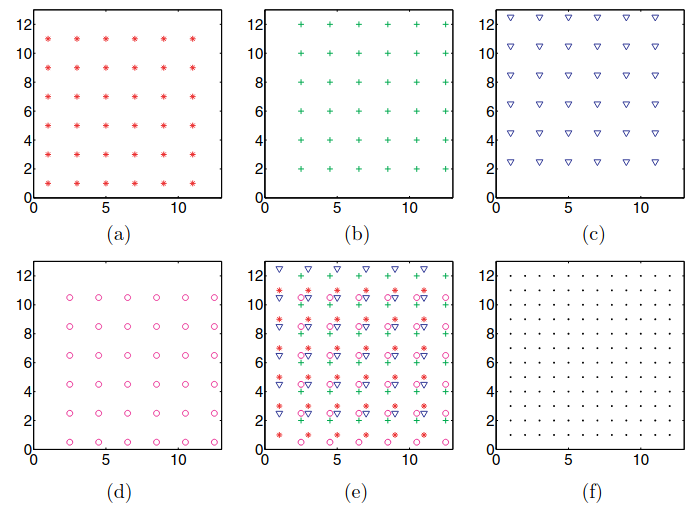
\includegraphics[width=4in]{classical-superresolution.png}
  \caption{Low-resolution images (a), (b), (c), and (d), when overlayed, sample the underlying phenomenon at the points in (e). This set of low-resolution images can synthesize a higher-resolution image, (f), with classical superresolution.}
  \label{classical-superresolution}
\end{figure}

However, in superresolution for simulations, the hidden variable is the high-granularity simulation, and it only exists discretely. There are no features in the high-granularity simulation to recover finer than the fine-grain gridpoints. This same theoretical justification does not apply, but perhaps another does: given the ergodic principle, every patch of space should have some patch in the training set that looks similar. In theory, superresolution can work by saving computational resources by learning what happens to small patches of space in the \textbf{training phase} and interpolating a novel patch based in the \textbf{prediction phase} (see \cref{gan-for-superresolution}a.). While neural networks are universal function approximators, a neural network can be more computationally expensive than the function it was trained to approximate (in this case, the fine-grained fluid dynamic simulation); in order to be worthwhile, high-resolution inference (\cref{gan-for-superresolution}b.) has to be cheaper than a bona fide high-resolution simulation (\cref{gan-for-superresolution}c.).

\begin{figure}[h!]
  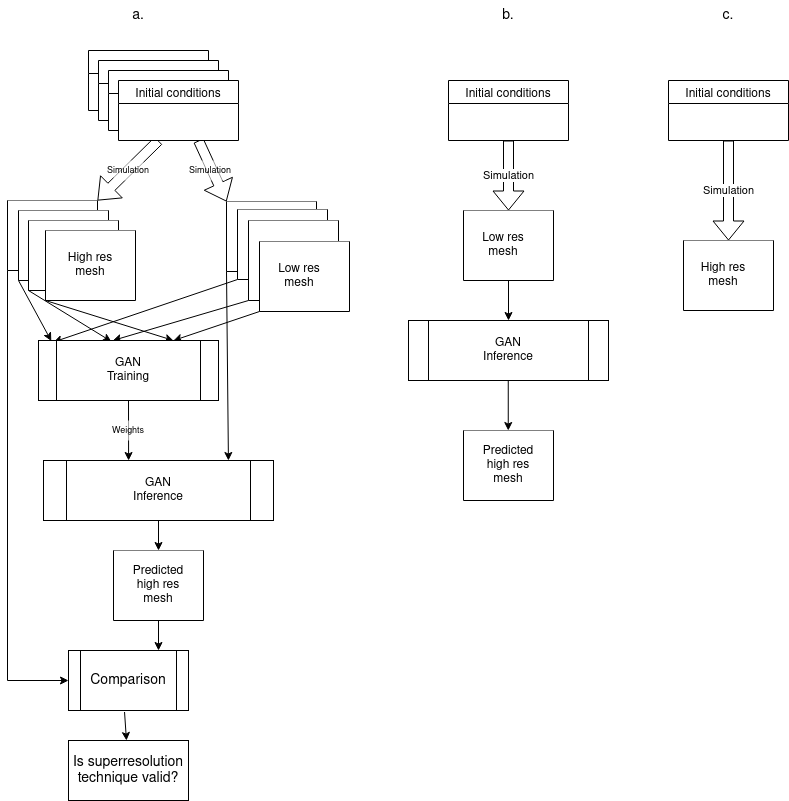
\includegraphics[width=\textwidth]{GAN_for_superresolution.drawio.png}
  \caption{a. shows training and validation of the GAN; b. shows usage of the GAN; c. shows the process the GAN can replace.}
  \label{gan-for-superresolution}
\end{figure}

Some \cite{superresolving-halos,survey} have suggested using a generative adverserial neural network (GAN) for superresolution. GANs were first proposed by Ian Goodfellow in 2014 \cite{GAN}. Suppose one wants to generate data in \(B\) based on a set of parameters \(A\). A GAN consists of two networks: a generator \(G: A \to B\) and a discriminator \(D: A \cross B \to [0, 1]\). To train a GAN, one needs genuine examples, \(R \subseteq A \cross B\). 
Intuitively, discriminator is trained to tell apart the genuine examples (elements of \(R\)), while the generator is trained to trick the descriminator with \((a, G(a))\) for \(a \in A\).
Let \[L(G, D) = \mathbb E [\log D(a, b) | (a, b) \in R] + \mathbb E [\log(1 - D(G(a))) | a \in A]\]
where \(\mathbb E(f(x) | x \in X)\) is the expected value of \(f(x)\).
Training runs in epochs where every even epoch updates the descriminator to maximize \(L\), while every odd epoch updates the generator to minimize \(L\), finding the \(\min\limits_G \max\limits_D L(G, D)\).

A Nash Equilibrium for this system is guaranteed to exist, although training might not reach it in a reasonable time. See \cite{GAN-explainer} for more background.
Once training is done, one can throw away \(D\) and use \(G\) to map from \(A\) to \(B\), hopefully in a realistic way.
In our case, \(A\) will be the low-resolution images, and \(B\) will be the high-resolution images.

Schaurecker et al. \cite{superresolving-halos} apply a generative adverserial network to superresolution for cosmological structure in a dark-matter simulation called Illustris \cite{Illustris}. Rather than an \textit{Eulerian} mesh, Illustris is based on a \textit{Lagrangian} unstructured mesh (aka moving mesh) code called Arepo \cite{Arepo}. It is an open question whether Eulerian mesh simulators would also benefit from the same superresolution techniques. Neural networks have hyperparameters, such as number of layers, number of neurons, and network architecture, which can make or break the application in practice \cite{hyperparameter-importance}. It is unclear if the hyperparameter choices in Schaurecker et al. for Illustris will transfer to a different simulator.

Schaurecker et al. \cite{superresolving-halos} use a descriminator that progressively downsamples the input with convlutional layers. Convultional layers are translationally invariant. For the generator, they use a U-net architecture introduced by \cite{unet} and adapted by \cite{unet-adaptation-1,unet-adaptation-2,unet-adaptation-3}. The basic idea behind the U-net is to generate an image by first generating high-level structure, then adding one level of detail based on that structure, and then one more (see \cref{unet}).However, the authors replace the up-sampling convolution by a tri-linear interpolation.

\begin{figure}[h!]
  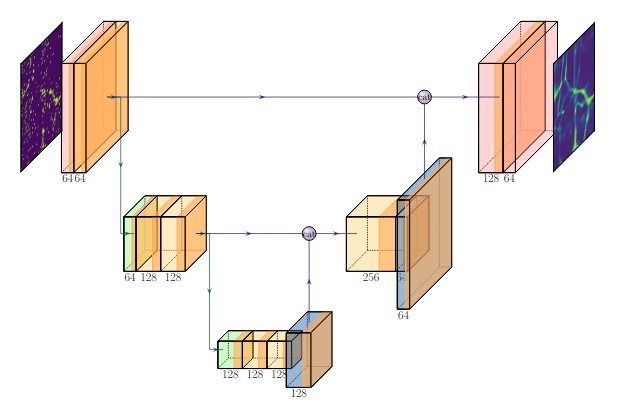
\includegraphics[width=\textwidth]{unet.png}
  \caption{U-net architecture used for the generator in \cite{superresolving-halos}. Note the three levels of hierarchy in generation.}
  \label{unet}
\end{figure}

Another hyperparameter in Schaurecker et al. is the objective function. Schaurecker et al. uses a regularization term suggested by \cite{GAN-regularization}
\[L(G, D) = \mathbb E [\log D(a, b) | (a, b) \in R] + \mathbb E [\log(1 - D(G(a))) | a \in A] + \gamma \mathbb E [\nabla D(a, b) | (a, b) \in R]\]
with \(\gamma = 5\). It is unclear if this hyperparameter will transfer to a different space.

\subsection*{Illustris and \textsc{AREPO}}

Illustris dataset\cite{nelson_illustris_2015,vogelsberger_introducing_2014} uses the \textsc{AREPO} solver, which evolves the fluid quantities according to the ``hyperbolic conservation laws of ideal hydrodynamics:''\cite{springel_e_2010}

\begin{tabular}{rl}
  \toprule
  State vector &
  \(\vb{U} = \mqty(\rho \\ \rho \vb{v} \\ \rho E)\) \\
  Flux &
  \(\vb{F}(\vb{U}) = \mqty(\rho \vb{v} \\ \rho \vb{v} \vb{v}^T + P \\ (\rho E + P) \vb{v})\) \\
  RHS &
  \(\vb{W} = \mqty(0 \\ -\frac{\dot{a}}{a} \rho \vb{v} - \frac{\rho}{a^2} \grad \phi \\ -2 \frac{\dot{a}}{a\rho E} - \frac{\rho \vb{v}}{a^2}\grad \phi \\)\) \\
  Evolution with time &
  \(\pdv{\vb{U}}{t} + \frac{1}{a} \div{\vb{F}} = \vb{W}\) \\
  Equation of state &
  \(P = (\gamma - 1) u\) \\
  Energy
  & \(E = u + \frac{1}{2} \rho v^2\) \\
  Gravitational potential & \(\grad^2 \phi = \frac{4 \pi G}{a} \rho_{\mathrm{total}} - \rho_0\) \\
\bottomrule
\end{tabular}

where \(\rho\) is the density field, \(\rho_0\) is the mean density field, \(\vb{v}\) is the velocity vector field, \(P\) is the pressure field, \(u\) is the internal energy field, \(a\) is the cosmological expansion constant, \(G\) is the gravitational constant, and \(\gamma\) is the ratio of specific heats, on an unstructured, moving, Voronoi tessellation mesh \cite{springel_e_2010}. \textsc{AREPO} is second order in space and second order in time, due to hierarchical adaptive time-stepping \cite{nelson_illustris_2015}.

\textsc{AREPO} uses Godunov's method in a MUSCL-Hancock scheme to solve these equations \cite{springel_e_2010}. The MUSCL-Hancock scheme is ``a slope-limited piece-wise linear reconstruction step within each cell, a first-order prediction step for the evolution over half a time-step, and finally a Riemann solver to estimate the time-averaged inter-cell fluxes for the time-step''\cite{van_leer_relation_1984,van_leer_upwind_2012}. Note that since the mesh is not cartesian, \textsc{AREPO} cannot employ operator splitting \cite{strang_construction_1968}.

\textsc{AREPO} uses Tree-PM (particle mesh) approach for computing self-gravity. Long-range forces are calculated using the Fourier particle-mesh method while short-range forces are computed with a hierarchical tree algorithm \cite{nelson_illustris_2015}.

The Illustris simulation further use Monte Carlo tracer particle scheme described in \cite{genel_following_2013}.

The Illustris initial conditions are set by running CAMB \cite{seljak_line--sight_1996} using parameters found in the Wilkinson Anisotropy probe \cite{hinshaw_nine-year_2013} or RECFAST \cite{seager_new_1999} (see \Cref{initial-conditions}).

\begin{table}[h]
\begin{tabular}{rl}
  \toprule
  \(\Omega_m\) & 0.2726 \\
  \(\Omega_\Lambda\) & 0.7274 \\
  \(\Omega_b\) & 0.0456 \\
  \(\sigma_8\) & 0.809 \\
  \(n_s\) & 0.963 \\
  \(H_0\) & 100 h km / sec Mpc \\
  \(h\) & 0.704 \\
  \(T(z = 157)\) & 245 K \\
  \bottomrule
\end{tabular}
\caption{Initial conditions for CAMB.}
\label{initial-conditions}
\end{table}

\subsection*{Enzo}

Enzo \cite{oshea_introducing_2004,bryan_enzo_2014} solves the magneto-hydrodynamics problem, in contrast to Illustris/\textsc{AREPO} which ignore magnetism. Enzo evolves the ``equations of ideal magnetohydrodynamics (MHD) including gravity, in a coordinate systems comoving with the cosmological expansion:''

\begin{tabular}{rl}
  \toprule
  State vector &
  \(\vb{U} = \mqty(\rho \\ \rho \vb{v} \\ \rho E)\) \\
  Flux &
  \(
  \vb{F}(\vb{U}) = \mqty(
  \rho \vb{v} \\
  \rho \vb{v} \vb{v}^T + P + \frac{B^2}{2a} - \frac{\vb{B} \vb{B}}{a} \\
  (\rho E + P + \frac{B^2}{2a}) \vb{v} - \frac{1}{a} \vb{B}(\vb{B} \cdot \vb{v}) \\
  )\) \\
  RHS & \(\vb{W} = \mqty(0 \\ -\frac{\dot{a}}{a} \rho \vb{v} - \frac{1}{a} \rho \grad \phi \\ -\frac{\dot{a}}{a} \qty(2 u - E - \frac{B^2}{2a}) - \frac{\rho}{a} \vb{v} \dot \grad \phi - \Lambda  + \Gamma + \frac{1}{a^2} \div{\vb{F}_{\mathrm{cond}}})\) \\
  Evolution with time &
  \(\pdv{\vb{U}}{t} + \frac{1}{a} \div{\vb{F}} = \vb{W}\) \\
  Equation of state &
  \(P = (\gamma - 1) u\) \\
  Energy
  & \(E = u + \frac{1}{2} \rho \vb{v}^2 + \frac{B^2}{2a}\) \\
  Maxwell's Equations & \(\pdv{\vb{B}}{t} - \frac{1}{a} \curl{(\vb{v} \cross \vb{B})} = 0\) \\
  Gravitational potential & \(\grad^2 \phi = \frac{4 \pi G}{a} \rho_{\mathrm{total}} - \rho_0\) \\
\bottomrule
\end{tabular}

where the variables are the same as in Illustris, but with magnetic vector field \(\vb{B}\), radiative cooling \(\Lambda\), radiative heating \(\Gamma\), and thermal heat conduction \(\vb{F}_{\mathrm{cond}}\). However, the situation I am simulating lacks a magnetic field anyway, so the extra magnetic capabilities won't matter. These equations are simulated on a  structured grid with adaptive mesh refinement \cite{bryan_enzo_2014}. Enzo takes adaptive timesteps. The order of accuracy depends on the spatial solver used in Enzo.

For a spatial solver, Enzo can use:
\begin{enumerate}
\item the hydrodynamic-only piecewise parabolic method (PPM) \cite{colella_piecewise_1984,bryan_piecewise_1995},
\item the MUSCL-like Godunov scheme \cite{van_leer_relation_1984,van_leer_upwind_2012},
\item a constrained transport (CT) staggered MHD scheme \cite{collins_cosmological_2010},
\item the second-order finite difference hydro-dynamics method described in ZEUS \cite{stone_zeus-2d_1992-1}
\end{enumerate}

Enzo uses cloud-in-cell (CIC) at half-time steps and the Fourier method to compute the gravitational field.

\subsection*{Applicability}

I am mostly not deciding which class of solvers to use, because I am wanting to reuse the neural network in \cite{schaurecker_super-resolving_2021} trained on Illustris data. Thus I am bound by the choices that Schaurecker et al. made in \cite{schaurecker_super-resolving_2021} and Nelson et al. in \cite{nelson_illustris_2015,vogelsberger_introducing_2014}. One in particular, Schaurecker chose to simulate dark-matter only. This is a coarser understanding of the universe, but it will be easier to process in a neural network.

\section*{Intermediate Results}

I am trying to use the same neural network architecture as Schaurecker et al.\cite{schaurecker_super-resolving_2021}. Schaurecker et al. have open sourced their code. \footnote{Source is available at \url{https://github.com/dschaurecker/dl_halo/}}

\begin{figure}[h!]
  \begin{centering}
    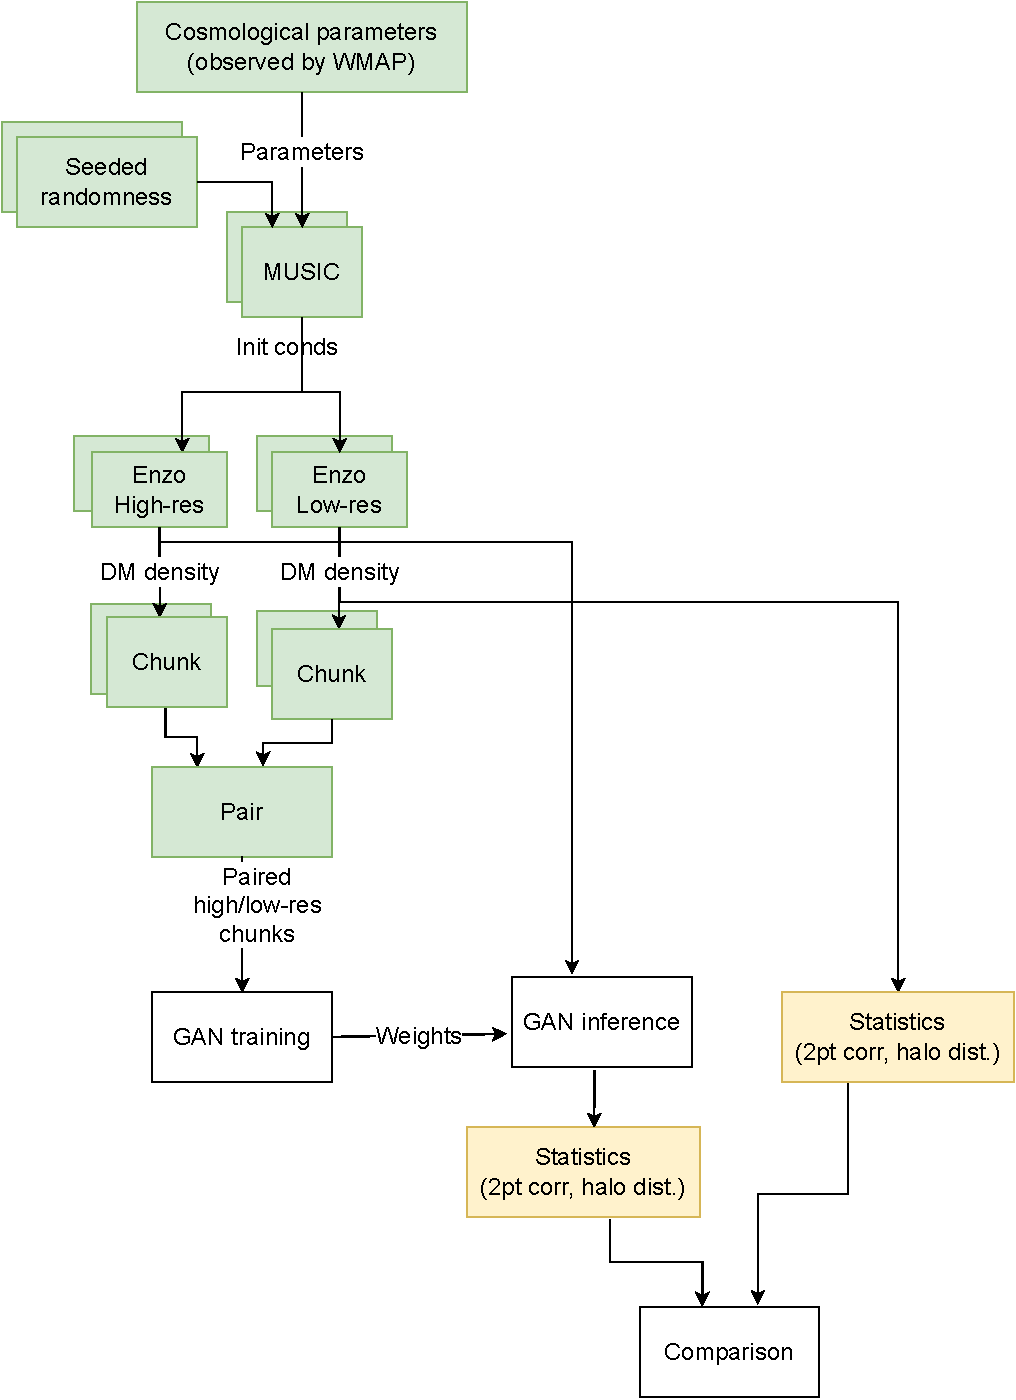
\includegraphics[width=0.7\textwidth]{./astrophysics-experiment-status.pdf}
  \end{centering}
  \caption{This figure shows the computational tasks in the experiment.}
  \label{workflow}
\end{figure}

Recall my experimental setup summarized in \cref{workflow}. I have written a script that can preform the green tasks in an automated fashion. I have partially implemented the yellow tasks. I have yet to implement the white tasks.

\begin{figure}[h!]
  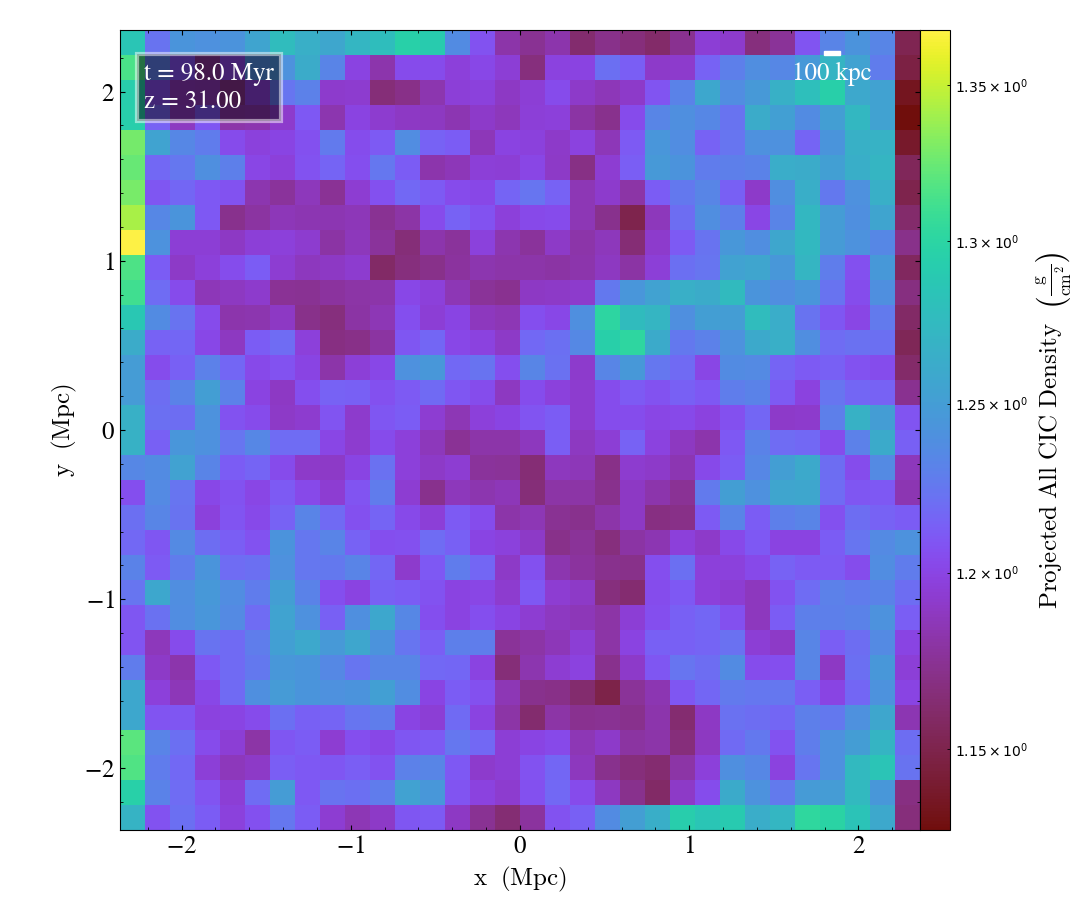
\includegraphics[width=0.45\textwidth]{../../presentation/assets/sim-0.png}
  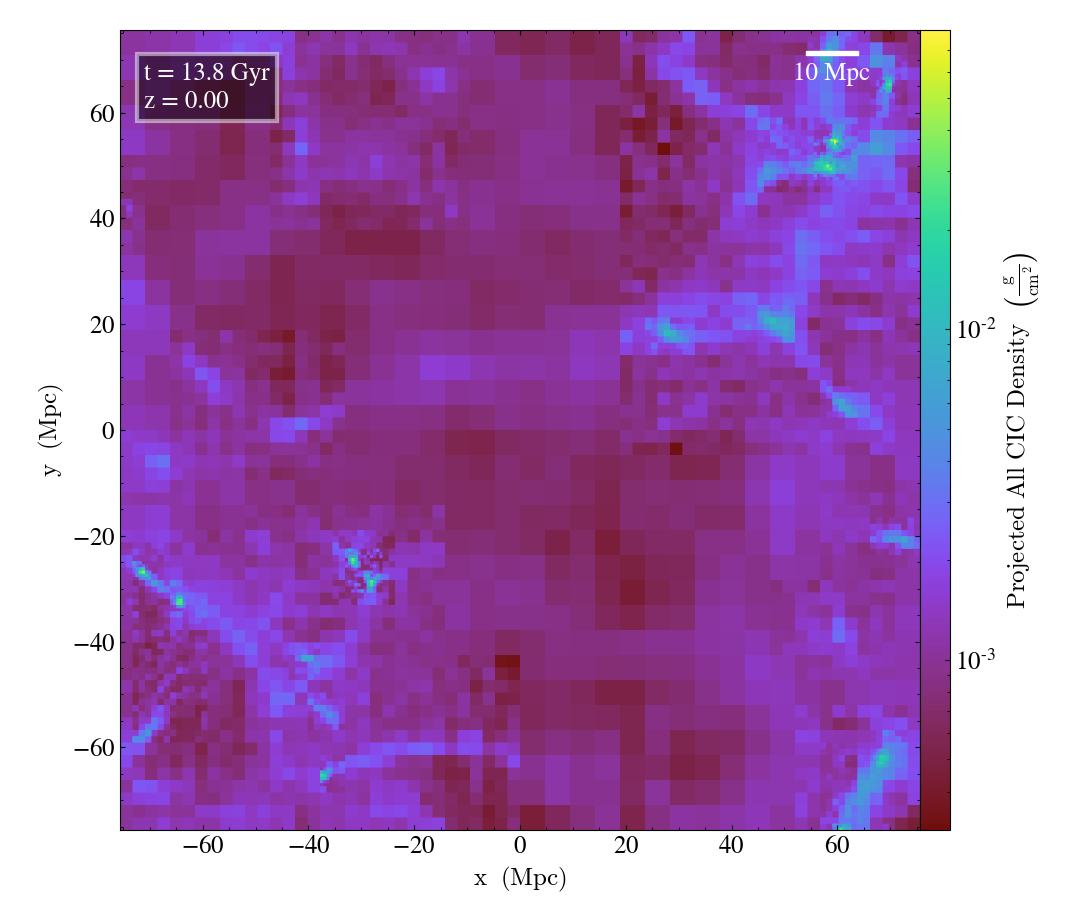
\includegraphics[width=0.45\textwidth]{../../presentation/assets/sim-1.png}
  \label{cosmology-result}
  \caption{This plot shows the dark matter density integrated along the Z-axis at the beginning of the simulation (left) and at the end (right) in comoving coordinates.}
\end{figure}

I believe that generating initial conditions with MUSIC \cite{hahn_multi-scale_2011} and simulating them with Enzo \cite{collins_cosmological_2010,bryan_enzo_2014} is working correctly based on the images in \cref{cosmology-result}. They show dark matter initially smeared out evenly across the universe (left figure) at z = 31, 98 Myr after the big bang. Then dark matter condenses into filaments and halos at z = 0, present day. One can see the adaptive mesh refine in ``interesting'' areas. Also note that the simulation region has physically expanded due to Hubble expansion.

% TODO: Low vs high res

\section*{Problems}

More work needs to be done to put the output of Enzo into a format that can be processed by the map2map\footnote{Source is available at \url{https://github.com/eelregit/map2map}} neural network library. Map2map requires that the AMR data be sampled desnely and split into equal-sized rectangular chunks with padding. 

I have been unable to install PyTorch on the campus cluster with CUDA. I have tried using the conda package manager, but it seems there is a diamond dependency conflict between the CUDA version of PyTorch and yt, another package I need to do this analysis.

Additionally, the FoaF halo finder requires the generated density field be resampled into individual particles. This is the opposite of CIC interpolation.

% TODO: Elaborate

\section*{Discussion}

\subsection*{Limitations of this approach}

Most well studied neural net operates on a field sampled at a regular grid, not an AMR grid. As such, the AMR output of Enzo has to be interpolated into a fixed grid. This ends up losing the advantages that the AMR had in the first place. If one uses the finest granularity everywhere, the sampling uses an extravagant amount of memory; if one uses a coarser resolution, the sampling fails to capture all of the details. This is particularly bad for cosmological simulations where there are extremely intricate halos and filaments surrounded by massive voids. It would be ideal if this neural networks could work natively on AMR grids, but this is a less well-studied case. With regular grids, we can reuse established building-blocks like the U-net and the concept of convolutional layers.

The prior literature \cite{schaurecker_super-resolving_2021,li_ai-assisted_2021} do not define explicit criteria for accepting or rejecting their superresolution approximation. They compare the power spectra, halo mass function, and halo two-point correlation functions graphically. It is difficult to know if an approximation is going to be acceptable without knowing what downstream analysis it is used in.

\subsection*{Simulation Applicability}

This approach to simulating cosmology relies on standard assumptions in \(\Lambda\)CDM. Following Schaurecker et al. \cite{schaurecker_super-resolving_2021}, this simulation neglects baryonic contributions to gravity formation. According to the Wilkinson Anisotropy Probe, baryonic matter only accounts for 4 -- 5\% of the mass-energy in the universe, while dark matter and dark energy accounts for the rest \cite{hinshaw_nine-year_2013}. Enzo assumes Newtonian gravity because the relativistic correction is small so long as the simulation size (100 Mpc ~ \(3 \times 10^{15}\) meters) is small compared to \(c / H = 1.4 \times 10^{26}\) meters) \cite{bryan_enzo_2014}.

\section*{Conclusion}

I successfully got Enzo working, and I learned a lot about the tools-of-the-trade for astrophysical simulation. More work can be done to integrate astrophysical toolkits like yt with neural network libraries like Keras and PyTorch. This would enable rapid development of neural network models for astrophysical simulation, which remains a promising direction.

\section*{Data Reproducibility}

I have attempted to make my code as reproducible as possible.

\begin{enumerate}
\item All of my source code is available here\footnote{\url{https://github.com/charmoniumQ/astrophysics-project}}, with a full revision history stored in Git.
\item I use the Spack package manager \cite{gamblin_spack_2015} to manage binary dependencies. Spack creates a `lockfile' which contains an exact specification of the source code and instructions to compile for every package. One can replicate my environment with \verb+spack env create myenv spack.lock+.
\item I use the Conda package manager to manage Python dependencies. Like Spack, this makes the software environment reproducible by others with \verb+conda env create --name myenv --file environment.yaml+.
\item I wrote detailed instructions in the \verb+README.md+ to set up my software.
\item I combined the complete workflow (simulation parameters all the way to grpahs) into a single script. However, the script knows to skip a task if the data already exists. This way, there are fewer steps, and the user doesn't need to manually run tasks of send the output of one task as the input to the next. Furthermore, the script can use ephemeral storage, such as \verb+/scratch+ on the Campus Cluster; If data gets deleted, it will just regenerate it.
\item I have each task is a function that gets called by the main script. This makes my code reusable in other tasks.
\item I wrote a library for running Slurm tasks on a remote machine and manipulating files on a remote machine. These can be resued in other tasks as well.
\end{enumerate}

